\section{Principal Component Analysis}  

  Say that we have a random vector $x = (x_1, \ldots, x_d)$. These $d$ covariates will naturally be correlated, and we want to ask whether some more fundamental set of independent variables exist \cite{1933hotelling} such that we can express
  \begin{equation}
    x = f(v_1, \ldots, v_k)
  \end{equation} 
  Naturally, we think of $f$ as a linear function. 

  We can think of PCA doing two things. First, it is a dimensionality-reduction algorithm where it takes samples $x \in \mathbb{R}^d$ and projects them into some smaller subspace $\mathcal{L}$ of dimension $k$. Second, it identifies an orthonormal basis of $\mathcal{L}$ that act as uncorrelated low-dimensional features. Because the projection map is linear and we are working in a lower-dimensional subspace, these new basis vectors are linear combinations of the original basis, which may reduce redundancy. Furthermore, by approximately modeling the original $x$ as a linear combination of these features, we are able to get a more parsimonious representation. 

  In PCA literature, it is more common to work with row vectors $x \in \mathbb{R}^{1 \times d}$, so linear mappings are realized through right matrix multiplication $x A$. Furthermore, we will assume that the data are $0$-mean. 

\subsection{L2 Residual Minimization Approach} 

  To give some motivation, we try to find a best fit line in $\mathbb{R}^d$. A line $\ell$ can be parameterized by a unit vector $v$ (note that it can be $\pm v$!), and so given some sample $x$, its projection onto $\ell$ is $\proj_{\ell} (x) = \langle x, v\rangle v$. Therefore, the residual is 
  \begin{align}
    \| x - \langle x, v \rangle v \|^2 & = \|x\|^2 - 2 \langle x, \langle x, v \rangle v \rangle + \| \langle x, v \rangle v \|^2 \\ 
                                       & = \|x\|^2 - 2 \langle x, v \rangle^2 + \langle x, v \rangle^2 \|v\|^2 \\ 
                                       & = \|x\|^2 - \langle x, v \rangle^2
  \end{align}
  since $\|v\|^2 = 1$ \cite{2019shalizi}. Now given a $0$-mean random variable $x$ (why we only consider $0$-mean RVs will be clear later), our risk is
  \begin{equation}
    R(v) = \mathbb{E}_x \big[ \| x - (x \cdot v) v \| \big] = \mathbb{E}_x \big[ \|x\|^2 \big] - \mathbb{E}_x \big[ \langle x, v \rangle^2 \big]
  \end{equation} 

  In practice, we want to minimize our empirical risk. Assume that we have sampled data $x^{(1)}, \ldots, x^{(n)} \sim x$. Then, 
  \begin{align} 
    \argmin_{v \in \mathbb{R}^{d}, \|v\| = 1} \hat{R}(v) 
    & =  \argmin_{v \in \mathbb{R}^{d}, \|v\| = 1} \frac{1}{n} \bigg( \sum_{i = 1}^n \|x^{(i)} \|^2 - \sum_{i=1}^n \langle x^{(i)}, v \rangle^2 \bigg) \\ 
    & = \argmax_{v \in \mathbb{R}^{d}, \|v\| = 1} \frac{1}{n} \sum_{i=1}^n \langle x^{(i)}, v \rangle^2 
  \end{align} 

  We have our loss function! Now what if we wanted to look for best fitting subspaces in general? Let's first rigorously define such a space. 

  \begin{definition}[Principal Subspace] 
    Let $x$ be a $0$-mean random variable in $\mathbb{R}^d$ and let $\mathcal{L}^k$ denote all $k$-dimensional linear subspaces of $\mathbb{R}^d$. The \textbf{$k$th principal subspace} is defined as 
    \begin{equation}
      \ell_k = \argmin_{\ell \in \mathcal{L}_k} \mathbb{E}_{\Tilde{x}} \big[ \| x - \proj_\ell x\|_2 \big]
    \end{equation}
  \end{definition}

  This isn't a big step from what we had before. We just want to construct a subspace $\ell$ that minimizes the expected $L^2$ distance between $x$ and $\ell$. Now how do we do such a thing? The most natural extension would be to identify an orthonormal basis $v_1, \ldots, v_k$, and since 
  \begin{equation}
    \proj_\ell x = \sum_{i=1}^k \proj_{v_i} x
  \end{equation} 
  our loss can be simplified to 
  \begin{align}
    R(\ell) = R(v_1, \ldots, v_k) 
    & = \mathbb{E} \bigg[ \| x - \proj_\ell x \|^2 \bigg] \\ 
    & = \mathbb{E} \bigg[ \|x\|^2 - 2 \langle x, \sum_{i=1}^k \proj_{v_i} x \rangle + \| \sum_{i=1}^k \proj_{v_i} x \|^2 \bigg] \\ 
    & = \mathbb{E} \bigg[ \|x\|^2 - 2 \sum_{i=1}^k \langle x, \proj_{v_i} x \rangle + \sum_{i=1}^k \| \proj_{v_i} x \|^2 \bigg] \\
    & = \mathbb{E} \bigg[ \|x\|^2 - 2 \sum_{i=1}^k \langle x, v_i \rangle^2 + \sum_{i=1}^k \langle x, v_i \rangle^2 \|v_i\|^2 \bigg] \\ 
    & = \mathbb{E} \bigg[ \|x\|^2 - \sum_{i=1}^k \langle x, v_i \rangle^2 \bigg] \label{loss}
  \end{align} 

  Now if $x$ was not $0$-mean, our intuition would tell us that the principal subspace should pass through its mean, or centroid. In fact \cite{1901pearson} showed this for a $1$-dimensional subspace. 

  \begin{lemma}[Principal Subspace Must Intersect Mean]
    Assume that $\mathbb{E}[x] \neq 0$, and by abuse of notation let us denote $\ell + p \in \mathbb{R}^d$ as the affine subspace $\ell$ that goes through $p$. 
    \begin{enumerate}
      \item If $p$ is orthogonal to $\ell$, then minimizes the risk is the average projection distance to the subspace. 
      \begin{equation}
        p = \mathbb{E}[x - \proj_\ell (x)]
      \end{equation}

      \item Another viable solution is 
        \begin{equation}
          p = \mathbb{E}_x [x]
        \end{equation}
        That is, $p$ must go through the mean of the data. 
    \end{enumerate}

    \begin{figure}[H]
      \centering 
      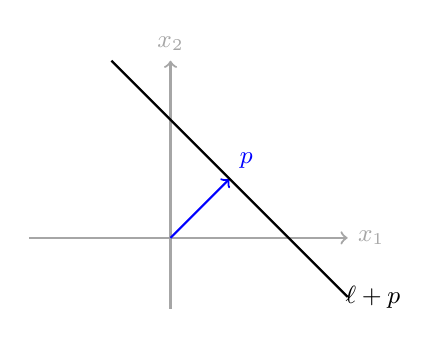
\begin{tikzpicture}[scale=1.5]
        % Axes
        \draw[->, thick, gray!70] (-1.2, 0) -- (1.5, 0) node[right] {\small $x_1$};
        \draw[->, thick, gray!70] (0, -0.6) -- (0, 1.5) node[above] {\small $x_2$};

        % Vector p
        \draw[->, thick, blue] (0,0) -- (0.5, 0.5) node[above right] {\small $p$};

        % Affine subspace l + p (orthogonal to p)
        \draw[thick] (-0.5,1.5) -- (1.5,-0.5);
        \node[] at (1.4,-0.5) [right] {\small $\ell + p$};
      \end{tikzpicture}
      \caption{By orthogonal intersection, we mean that for any $w \in \ell$, $\langle w, p \rangle = 0$} 
    \end{figure}
  \end{lemma}
  \begin{proof}
    We actually free $p$ to be any vector, not necessarily orthogonal. The projection distance of $x$ onto $\ell + p$ is the same as the projection distance from $x-p$ onto $\ell$. Therefore, $v_i$'s are orthogonal, we can derive
    \begin{align}
      R(\ell, p) & = \mathbb{E}_x \big[ \| x - \proj_{\ell + p} (x) \|^2 \big] \\ 
                 & = \mathbb{E}_x \big[ \| (x - p) - \proj_\ell (x - p) \|^2 \big] \\
                 & = \mathbb{E}_x \bigg[ \|x - p\|^2 + \bigg\| \sum_{i=1}^k \proj_{v_i} (x - p) \bigg\|^2 - 2 \Big\langle x - p, \sum_{i=1}^k \proj_{v_i} (x - p) \Big\rangle \bigg] \\ 
                 & = \mathbb{E}_x \bigg[ \|x - p\|^2 - \sum_i \langle x - p, v_i \rangle^2 \bigg] 
    \end{align}
    To find the minimum, we take the total derivative and set it equal to $0$. We are taking the derivative w.r.t. $p$ of an integral w.r.t. $x$, so we can push the derivative into the integral and solve. 
    \begin{align}
      0 = \frac{\partial R(\ell, p)}{\partial p} 
        &= \mathbb{E}_x \left[ \frac{\partial}{\partial p} \left\{ \|x - p\|^2 - \sum_i \langle x - p, v_i \rangle^2  \right\} \right] \\
        &= \mathbb{E}_x \left[ 2(p - x) + 2 \sum_{i=1}^k \langle x - p, v_i \rangle v_i \right]  \\ 
        &= \mathbb{E}_x \left[ 2(p - x) + 2 \proj_{\ell} (x - p) \right]
    \end{align} 
    This has an infinite number of solutions, but by constraining $p$ to be orthogonal to $\ell$, we can get a unique one. In this case, $\proj_\ell (x - p) = \proj_\ell (x)$ and we have 
    \begin{equation}
      p = \mathbb{E}_{x} [x - \proj_\ell (x)]
    \end{equation}
    Or, we can simply substitute $p = \mathbb{E}_x [x]$ and see that everything cancels out. 
  \end{proof}

  Therefore, we can just normalize the data to $0$ and simply use \ref{loss} without having to account for the affine translation $p$. In the empirical case, we can get rid of the fixed $x$ and find 
  \begin{equation}
    \argmax_{v_i \in \mathbb{R}^d} \frac{1}{n} \sum_{j=1}^n \sum_{i=1}^k \langle x^{(j)}, v_i \rangle^2, \quad \text{ subject to } \|v_i\|^2 = 1, \langle v_i, v_j \rangle = 0 \text{ for } i \neq j
  \end{equation} 

  By stacking the $v_i$'s left-to-right in matrix $V_k \in \mathbb{R}^{d \times k}$, we can get a cleaner form of the loss function. 
  \begin{align}
    \frac{1}{n} \sum_{j=1}^n \sum_{i=1}^k \langle x^{(j)}, v_i \rangle^2 
    & = \frac{1}{n} \sum_{j=1}^n \sum_{i=1}^k (x^{(j)})^T v_i v_i^T x^{(j)} \\ 
    & = \frac{1}{n} \sum_{j=1}^n (x^{(j)})^T V_k V_k^T x^{(j)} \\ 
    & = \frac{1}{n} \Tr(X V_k V_k^T X^T) = \frac{1}{n} \Tr(V_k^T X^T  X V_k) \label{trace}
  \end{align}
  This leads to an intuitive loss function for PCA. 

  \begin{theorem}[Constrained Empirical Risk of $k$th Principal Subspace]
    The empirical risk, or loss function, of PCA is
    \begin{equation}
      \argmax_{V \in \mathbb{R}^{d \times k}, V_k^T V_k = I_k} 
      \frac{1}{n} \| X - X V_k V_k^T\|^2
    \end{equation}
  \end{theorem} 
  \begin{proof}
    By the Frobenius norm expansion and since $V_k^T V_k = I_k$, we have 
    \begin{align}
      \|X - X V_k V_k^T\|_F^2 
      & = \Tr((X - X V_k V_k^T)^T(X - X V_k V_k^T)) \\
      & = \Tr(X^T X - X^T X V_k V_k^T - V_k V_k^T X^T X + V_k V_k^T X^T X V_k V_k^T) \\
      & = \Tr(X^T X) - 2\Tr(X^T X V_k V_k^T) + \Tr(V_k V_k^T X^T X V_k V_k^T) \\ 
      & = \Tr(X^T X) - 2\Tr(V_k^T X^T X V_k) + \Tr(V_k^T V_k V_k^T X^T X V_k) \\
      & = \Tr(X^T X) - 2\Tr(V_k^T X^T X V_k) + \Tr(V_k^T X^T X V_k) \\ 
      & = \Tr(X^T X) - \Tr(V_k^T X^T X V_k) 
    \end{align}
    and since the empirical risk does not depend on $X$, minimizing the Frobenius norm is equivalent to maximizing the second trace term, i.e. \ref{trace}. 
  \end{proof}

  \begin{definition}[Projection Operator]
    Note that there are two distinct projection operators, which are realized through right matrix multiplication. 
    \begin{enumerate}
      \item The linear map $V_k : \mathbb{R}^d \to \mathbb{R}^k$ is a projection operator of the samples $x$ into the component space. 
      \item The linear map $V_k V_k^T : \mathbb{R}^d \to \mathbb{R}^d$ is called the \textbf{rank-k projection operator} onto the $k$th principal subspace. 
    \end{enumerate}
  \end{definition}

  Therefore, $X V_k \in \mathbb{R}^{n \times k}$ is the projection of the dataset into the component space. If we want to get the denoised samples in the sample space $\mathbb{R}^d$, we project it back out $X V_k V_k^T$. 

\subsection{Variance Maximization Approach}

  But we can turn this into a variance maximization problem. Note that $\Var_x [\langle x, v \rangle] = \mathbb{E}_x [ \langle x, v \rangle^2 ] - \mathbb{E}_x [ \langle x, v \rangle]^2$, and so we can rewrite our true risk as 
  \begin{align}
    \argmin_{v \in \mathbb{R}^d, \|v\|=1} R(v) = \argmin_{v \in \mathbb{R}^d, \|v\|=1} \mathbb{E}_x \big[ \|x\|^2 \big] - \Var_x [\langle x, v \rangle] - \mathbb{E}_x [ \langle x, v \rangle]^2
  \end{align} 
  where the last term vanishes since $x$ is $0$-mean, and hence by linearity of expectation $\mathbb{E}_x [\langle x, v \rangle] = \langle \mathbb{E}[x], v \rangle = \langle 0, v \rangle = 0$. In parallel the empirical risk reduces to simply the sample variance. 
  \begin{equation}
    \argmax_{v \in \mathbb{R}^{d}, \|v\| = 1} \hat{\Var}[ \langle x, v \rangle] = \argmax_{v \in \mathbb{R}^{d}, \|v\| = 1} \frac{1}{n} \bigg( \sum_{i=1}^n \langle x^{(i)}, v \rangle^2 \bigg)
  \end{equation} 

  Therefore, we can think of the $L^2$ minimization problem as equivalent to a variance maximization approach.  

  \begin{lemma}[Variance Maximization Approach]
    Minimizing the $L^2$ distance of a random variable $x$ to a line $\ell$ in $\mathbb{R}^d$ is equivalent to maximizing the scalar variance in the projected space. 
    \begin{equation}
      \argmin_{v \in \mathbb{R}^d, \|v\| = 1} \mathbb{E} [ \| x - \proj_v (x) \|_2 ] = \argmax_{v \in \mathbb{R}^d, \|v\| = 1} \Var_x [\langle x, v \rangle ]
    \end{equation}
  \end{lemma}

  \begin{figure}[H]
    \centering
    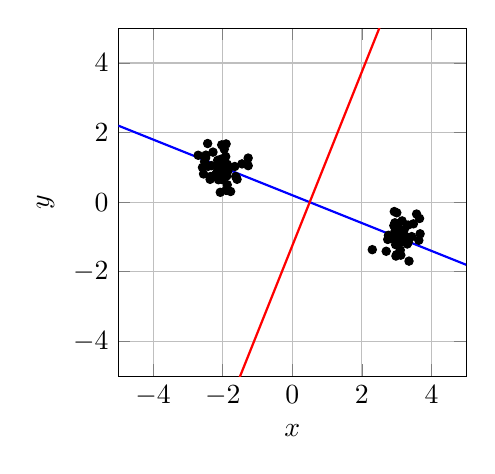
\begin{tikzpicture}
      \begin{axis}[
        xlabel={$x$}, ylabel={$y$},
        axis equal,
        xmin=-5, xmax=5,
        ymin=-5, ymax=5,
        grid=both,
        width=6cm, height=6cm
      ]
      
      \foreach \i in {1,...,50} {
        \pgfmathsetmacro\x{-2 + 0.8*rnd*cos(360*rnd)}
        \pgfmathsetmacro\y{1 + 0.8*rnd*sin(360*rnd)}
        \addplot[only marks, mark=*, mark size=1.5pt, color=black] coordinates {(\x,\y)};
      }
      
      \foreach \i in {1,...,50} {
        \pgfmathsetmacro\x{3 + 0.8*rnd*cos(360*rnd)}
        \pgfmathsetmacro\y{-1 + 0.8*rnd*sin(360*rnd)}
        \addplot[only marks, mark=*, mark size=1.5pt, color=black] coordinates {(\x,\y)};
      }

      % Line from (-2,1) to (3,-1): slope -2/5
      \addplot[thick, blue, domain=-5:5, samples=2] {-0.4*(x + 2) + 1};

      % Perpendicular line through midpoint (0.5, 0), slope 5/2
      \addplot[thick, red, domain=-5:5, samples=2] {2.5*(x - 0.5)};
      \end{axis}
    \end{tikzpicture}
    \caption{Projecting the dataset onto the blue line seems to retain more variance than projecting onto the red line.}
  \end{figure}

  Let's in fact try to directly maximize the variance. If we vertically stack our $n$ data points into a matrix $X \in \mathbb{R}^{n \times d}$, then the projections of this data onto $\mathbb{R}$ is simply $X v \in \mathbb{R}^n$. Again, since this is $0$-mean, the variance is 
  \begin{align}
    \label{eq:var_decom}
    \hat{\Var}(Xv) 
    & = \frac{1}{n} (Xv)^T (Xv) \\ 
    & = \frac{1}{n} v^T X^T X v \\
    & = v^T \frac{X^T X}{n} v \\ 
    & = v^T \hat{\Sigma} v
  \end{align}
  where $\hat{\Sigma}$ is the empirical covariance matrix of $X$. We want to find 
  \begin{equation}
    \max_{v} v^T \hat{\Sigma} v \text{ subject to } \|v\|^2 = 1
  \end{equation} 
  This is a classic Lagrange multiplier problem. We construct the Lagrangian and compute its partial derivatives to set equal to $0$. 
  \begin{align}
    \mathcal{L}(v, \lambda) & = v^T \hat{\Sigma} v - \lambda (\|v\|^2 - 1) \\  
    \frac{\partial \mathcal{L}}{\partial v} & = 2 \hat{\Sigma} v - 2 \lambda v = 0 \\ 
    \frac{\partial \mathcal{L}}{\partial \lambda} & = v^T v - 1 = 0
  \end{align} 
  which gives us 
  \begin{equation}
    \hat{\Sigma} v = \lambda v, \qquad v^T v = 1
  \end{equation} 
  This tells us that $v$ is a unit eigenvector, and the maximizing vector will be the one corresponding to the largest eigenvalue. Essentially, we have reduced this to an eigenvalue problem. 
  
  \begin{theorem}[1st Principal Subspace as Eigenvector]
    The first principal subspace of data matrix $X \in \mathbb{R}^{n \times d}$ is spanned by the eigenvector corresponding to the largest eigenvalue of the sample covariance matrix $\hat{\Sigma} = \frac{1}{n} X^T X$. 
  \end{theorem}

  Now for higher dimensional subspaces, we take the same approach. Going through the same derivation gives the expected risk in terms of the variance 
  \begin{align}
    R(v_1, \ldots, v_k) 
    & = \mathbb{E}[\|x\|^2] - \sum_{i=1}^k \mathbb{E}[ \langle x, v_i \rangle^2 ] \\ 
    & = \mathbb{E}[\|x\|^2] - \sum_{i=1}^k \Var[\langle x, v_i \rangle ] - \mathbb{E}[ \langle x, v_i \rangle ]^2 
  \end{align} 
  By fixing the $x$'s and going through the same derivation as \ref{eq:var_decom}, we get our equivalent empirical risk. 
  \begin{equation}
    \argmax_{v_i \in \mathbb{R}^d} \sum_{i=1}^k \hat{\Var}[\langle x, v_i \rangle] = \argmax_{v_i \in \mathbb{R}^d} \sum_{i=1}^k v_i^T \hat{\Sigma} v_i
  \end{equation}

  \begin{theorem}[Constrained Empirical Risk of $k$th Principal Subspace]
    The empirical risk tells us to find an orthonormal basis that maximizes the sum of the variance of projections. 
    \begin{equation}
      \argmax_{v_i \in \mathbb{R}^d} \sum_{i=1}^k  v_i^T \hat{\Sigma} v_i \text{ subject to } \|v_i\|^2 = 1, \langle v_i, v_j \rangle = 0 \text{ for } i \neq j
    \end{equation}
  \end{theorem}

  The variance-maximization loss is very insightful, and we may naively think of just taking the unit eigenvectors corresponding to the top $k$ largest eigenvalues. Surprisingly, this greedy approach turns out to be correct. 

  Let's derive this further 
  \begin{align}
    \sum_{i = 1}^k v_i^T \hat{\Sigma} v_i 
    & = \sum_{i=1}^k \Tr(v_i v_i^T \hat{\Sigma}) \\ 
    & = \Tr(V_k V_k^T \hat{\Sigma}) \\ 
    & = \Tr(\hat{\Sigma} V_k V_k^T)
  \end{align}
  which again is equal to \ref{trace}. By the spectral theorem, we can take the eigendecomposition of self-adjoint $\hat{\Sigma} = Q \Lambda Q^T$ with orthogonal matrix $Q$. Setting $W_k = Q^T V_k$, we have 
  \begin{equation}
    \Tr(\hat{\Sigma} V_k V_k^T) = \Tr(Q \Lambda Q^T V_k V_k^T) = \Tr(\Lambda Q^T V_k V_k^T Q) = \Tr(\Lambda W_k W_k^T) = \sum_{i = 1}^d \lambda_i (W_k W_k^T)_{ii}
  \end{equation}
  where without loss of generality we have $\lambda_1 \geq \lambda_2 \geq \ldots \geq \lambda_d$. However, we have two constraints. First, since $W_k W_k^T$ is a projection matrix, the eigenvalues must be between $0$ and $1$. Second, by the cyclic trace property, we have $\Tr(W_k W_k^T) = \Tr(I_k) = k$.\footnote{Though it is \textit{not} the case that $W_k W_k^T = I_k$!} So denoting $w_i = (W_k W_k^T)_{ii}$, we have the optimal allocation problem 
  \begin{equation}
    \max \sum_{i=1}^d \lambda_i w_i \text{ subject to } \begin{cases} 
      w_i \in [0, 1] \; \forall i = 1, \ldots, d \\
      \sum_i w_i = k
    \end{cases}
  \end{equation}
  Since the eigenvalues are decreasing, it doesn't take too much to see that the optimal solution is to just put everything you have into the largest eigenvalues. So we fill the first $w_1 = \ldots = w_k = 1$ and the rest $w_{k+1}, \ldots w_d = 0$. Therefore, this solution corresponds to $W_k = (e_1, e_2, \ldots, e_k)$, and so 
  \begin{equation}
    V_k = Q W_k = Q_k
  \end{equation}
  which is the truncated matrix $Q$ containing the first $k$ eigenvectors of $\hat{\Sigma}$ corresponding to the largest eigenvalues. At this point, it does not suffice to talk about just a principal subspace anymore. We must identify its orthonormal basis, i.e. the eigenvectors. 

  \begin{definition}[Principal Axis]
    The eigenvectors $v_1, \ldots, v_k$ that span the $k$th principal subspace are called the top $k$ \textbf{principal axes}, or \textbf{principal directions}.\footnote{The terminology is misused and confusing sometimes. See \href{https://stats.stackexchange.com/questions/88118/what-exactly-is-called-principal-component-in-pca}{https://stats.stackexchange.com/questions/88118/what-exactly-is-called-principal-component-in-pca}.} 
  \end{definition} 
  
  \begin{definition}[Principal Scores]
    Given a sample $x \in \mathbb{R}^d$, its top $k$ \textbf{principal scores} are defined in the equivalent ways. It is basically the coefficients of reduced-rank approximation with respect to the basis spanned by the principal axis. 
    \begin{enumerate}
      \item It is the components of $V_k^T x$. That is, we take a sample and project it onto the component space. 
      \begin{equation}
        x = \sum_i a_i e_i \mapsto V_k^T x = \sum_j b_j e_j^
        \prime
      \end{equation} 
      where $e_i, e_j^\prime$ are the basis vectors in $\mathbb{R}^d, \mathbb{R}^k$. Then $b_1, \ldots, b_k$ are the principal scores of $x$. 

      \item It is the coefficients of $x$ with respect to the basis spanned by the top $k$ eigenvalues. 
      \begin{equation}
        x = c_1 v_1 + c_2 v_2 + \ldots + c_k v_k + c_{k+1} v_{k+1} + \ldots + c_d v_d
      \end{equation} 
      Then $c_1, \ldots, c_k$ are the principal scores. 

      \item Though we haven't introduced SVD here, it turns out to be equivalent to $x^T V_k^T$ is equivalent to $US_k$. 
    \end{enumerate}
  \end{definition}
  \begin{proof}
    These two are clearly equivalent since 
    \begin{equation}
      b_1 e_1^\prime + \ldots + b_k e_k^\prime = V_k^T x = V_k^T \left( \sum_{i=1}^d c_i v_i \right) = \sum_{i=1}^d c_i V_k^T v_i = \sum_{i=1}^k c_i e_i^\prime 
    \end{equation} 
    which is of the proper form when $c_i = b_i$. Since $V_k^T$ is a truncated orthogonal matrix, $V_k^T v_i = e_i^\prime$ for $1 \leq i \leq k$ and $0$ for all else. 
  \end{proof}

  This is similar to taking the first principal component $v_1$ on $X$, and then by computing the first principal component on the remaining residuals $X - \proj_{v_1} X$, we get the second principal component, which is guaranteed to be orthogonal. But usually, we end up just computing all eigenvectors at once. 

  Now how do we know that this sample decomposition is a good approximation to the true decomposition? It comes from the fact that the sample covariance $\hat{\Sigma}$ is a good approximation of the true covariance $\Sigma$, which we will later prove using concentration of measure. 

  \begin{theorem}[Risk]
    The risk satisfies 
    \begin{equation}
      R(k) = \mathbb{E}[\| x - V_k V_k^T x \|^2 ] = \sum_{j=k+1}^D \lambda_j 
    \end{equation}
  \end{theorem}

  It is essential that you plot the spectrum in decreasing order. This allows you to analyze how well PCA is working. People often use the ``elbow'' technique to determine where to choose $K$, and we value 
  \begin{equation}
    \frac{\sum_{j=1}^k \lambda_j}{\sum_{j=1}^d \lambda_j} 
  \end{equation}
  accounts for the \textbf{variance explained}, which should be high with $K$ low. If you have to go out to dimension $K=50$ to explain $90\%$ of the variance, then PCA is not working. It may not work because of many reasons, such as there being nonlinear structure within the data. 

\subsection{Decomposition Solvers}

  So far, the equivalence of the L2 minimization approach and variance maximization approach had been firmly established by 1933 in \cite{1933hotelling}. However, the person who formalized the connection in using low-rank approximations in PCA was Eckart and Young in 1936 \cite{1936eckart}.\footnote{In fact, a stronger version was proved before, but they rediscovered it.}
  
  \begin{theorem}[Eckart-Young Theorem]
    The solution to 
    \begin{equation}
      \min_{A_k \in \mathbb{R}^{m \times n}} \| A - A_k \|_F, \qquad \text{ subject to } \mathrm{rank}(A_k) \leq k
    \end{equation} 
    is given by the matrix $A_k = U S V_k^T$, where $A = U S V^T$ is the singular value decomposition of $A$, and $V_k$ is the truncated matrix formed from the first $k$ columns of $V$. Note that $\| \cdot \|_F$ is the Frobenius norm. 
  \end{theorem}
  \begin{proof}
    Let $A \in \mathbb{R}^{m \times n}$ be a real (possibly rectangular) matrix with $m \leq n$. Suppose that
    \begin{equation}
      A = U\Sigma V^T
    \end{equation}
    is the singular value decomposition of $A$.

    We claim that the best rank $k$ approximation to $A$ in the Frobenius norm, denoted by $\| \cdot \|_F$, is given by
    \begin{equation}
      A_k = \sum_{i=1}^k \sigma_i u_i v_i^T
    \end{equation}
    where $u_i$ and $v_i$ denote the $i$th column of $U$ and $V$, respectively.

    First, note that we have
    \begin{equation}
      \|A - A_k\|_F^2 = \left\|\sum_{i=k+1}^n \sigma_i u_i v_i^T\right\|_F^2 = \sum_{i=k+1}^n \sigma_i^2
    \end{equation}

    Therefore, we need to show that if $B_k = XY^T$ where $X$ and $Y$ have $k$ columns then
    \begin{equation}
      \|A - A_k\|_F^2 = \sum_{i=k+1}^n \sigma_i^2 \leq \|A - B_k\|_F^2.
    \end{equation}

    By the triangle inequality with the spectral norm, if $A = A' + A''$ then $\sigma_1(A) \leq \sigma_1(A') + \sigma_1(A'')$. Suppose $A_k'$ and $A_k''$ respectively denote the rank $k$ approximation to $A'$ and $A''$ by SVD method described above. Then, for any $i, j \geq 1$
    \begin{align}
      \sigma_i(A') + \sigma_j(A'') &= \sigma_1(A' - A'_{i-1}) + \sigma_1(A'' - A''_{j-1}) \\
      &\geq \sigma_1(A - A'_{i-1} - A''_{j-1}) \\
      &\geq \sigma_1(A - A_{i+j-2}) \quad \text{(since $\text{rank}(A'_{i-1} + A''_{j-1}) \leq i + j - 2$)} \\
      &= \sigma_{i+j-1}(A).
    \end{align}

    Since $\sigma_{k+1}(B_k) = 0$, when $A' = A - B_k$ and $A'' = B_k$ we conclude that for $i \geq 1, j = k + 1$
    \begin{equation}
      \sigma_i(A - B_k) \geq \sigma_{k+i}(A).
    \end{equation}

    Therefore,
    \begin{equation}
      \|A - B_k\|_F^2 = \sum_{i=1}^n \sigma_i(A - B_k)^2 \geq \sum_{i=k+1}^n \sigma_i(A)^2 = \|A - A_k\|_F^2,
    \end{equation}
    as required.
  \end{proof}

  Now this gives the theoretical justificiation to use SVD. Since $\frac{1}{n} X^T X = \frac{1}{n} V S U^T U \sigma V^T = \frac{1}{n} V S^2 V^T$, the columns of $V$ are the principal axes. Recall from linear algebra that $\Lambda = S^2$. 

  \begin{theorem}[Principal Scores]
    The top $k$ principal scores of a dataset $X = U S V^T$ is simply  
    \begin{equation}
      U S_k
    \end{equation}
    where $S_k \in \mathbb{R}^{d \times k}$ is $S$ truncated after the first $k$ columns. 
  \end{theorem}
  \begin{proof}
    Remember that for a single sample $x$, its score was $V^T x$. In row-form, we have $x V$, and taking into account the whole dataset, we have $XV$. But 
    \begin{equation}
      XV = U S V^T V = US
    \end{equation}
    and by truncating the $k$th principal components, we have our result.  
  \end{proof}

  \begin{algo}[PCA with SVD] 
    Given a dataset $X \in \mathbb{R}^{n \times d}$, let us denote the rows as $x_i$, and say that we are looking for a subspace of dimension $k$. 
    \begin{enumerate}
      \item Compute the mean 
      \begin{equation}
        \mu = \frac{1}{n} \sum_{i=1}^n x_i  \in \mathbb{R}^d
      \end{equation} 

      \item Standardize the data $\Tilde{X} = X - \mu$, i.e. $\Tilde{x}_i = x_i - \mu$.  

      \item Compute the SVD $\Tilde{X} = U S V^T$.

      \item Compute the submatrices $V_k \in \mathbb{R}^{k \times k}$ and $S_k \in \mathbb{R}^{D \times k}$. 

      \item Define the projection operator $P_k (x) = \mu + \sum_{j=1}^k \langle x - \mu, v_j \rangle \, v_j$, the change of basis operator $T$, and the embedding operator $T^{-1} (z) = \mu + V_k S_k z$. 
    \end{enumerate} 
    A demonstration is done \href{code/pca.html}{here}.
  \end{algo}

  \begin{example}[Walkthrough]
    Say that we have some dataset of 100 points in $\mathbb{R}^3$. The data matrix is shown on the right, but in reality I just generated a toy dataset. 

    \noindent\begin{minipage}{.5\textwidth}
      \begin{lstlisting}[]{Code}
        def scatter(n=1000): 
          X_2d = np.random.multivariate_normal(
            np.zeros(2), np.eye(2), n) 
          A = np.array([[1, 1, 1], [-2, 2, 1]])
          X_3d = X_2d @ A + np.random.multivariate_normal(
            np.zeros(3), np.eye(3), n)
          return X_3d
      \end{lstlisting}
      \end{minipage}
      \hfill
      \begin{minipage}{.49\textwidth}
      \begin{lstlisting}[]{Output}
        [[ 8.864e-01  3.975e-01  7.009e-01]
         [-2.065e+00  3.258e+00  1.874e+00]
         [ 3.970e-01 -5.400e-01 -3.054e-01]
         [ 3.239e+00 -1.999e+00 -1.034e+00]
         ...
         [-1.295e-01  9.683e-01  2.861e-01]
         [-7.097e-01 -4.060e-01 -1.058e+00]
         [ 2.284e+00 -2.505e+00 -1.522e+00]]
      \end{lstlisting}
    \end{minipage}

    We can take the SVD, which will give us

    \begin{lstlisting}
      In [7]: U, S, Vt = np.linalg.svd(X)

      In [8]: print(U)
      [[ 4.804e-04  7.852e-02  4.071e-02 ...  5.320e-03  5.034e-02 -9.305e-02]
       [ 1.420e-01  3.992e-02 -1.229e-02 ... -5.512e-02  4.460e-02  7.192e-02]
       [-2.456e-02 -3.657e-03 -4.578e-04 ... -1.005e-01 -1.512e-01 -7.300e-02]
       ...
       [ 2.909e-02  2.754e-02 -1.075e-01 ...  9.871e-01 -1.325e-02 -3.559e-03]
       [-8.714e-03 -8.159e-02 -1.436e-01 ... -1.297e-02  9.733e-01 -1.055e-02]
       [-1.241e-01  2.077e-03 -6.028e-02 ... -3.435e-03 -8.286e-03  9.819e-01]]

      In [9]: print(S)
      [29.90178039 15.17454164  3.01267412]

      In [10]: print(Vt.T)
      [[-0.59855644  0.77282378 -0.21088764]
       [ 0.70716875  0.38606989 -0.59233639]
       [ 0.37635428  0.50367991  0.77760144]] 
    \end{lstlisting} 

    The \texttt{Vt.T} represents $V$, with its columns being our principal axes, and we wish to plot them along with our data points. We would like to scale them by their variance captured. 
    \begin{enumerate}
      \item Take the singular values $(\sigma_1, \sigma_2, \sigma_3) = (29.9, 15.2, 3.0)$. 
      \item Square them to get the eigenvalues $(\lambda_1, \lambda_2, \lambda_3) = (894, 230, 9)$. 
      \item Normalize them to get the percent variance captured. $(0.789, 0.203, 0.008)$, and use this as a scale for each eigenvector. 
    \end{enumerate}

    \begin{figure}[H]
      \centering 
      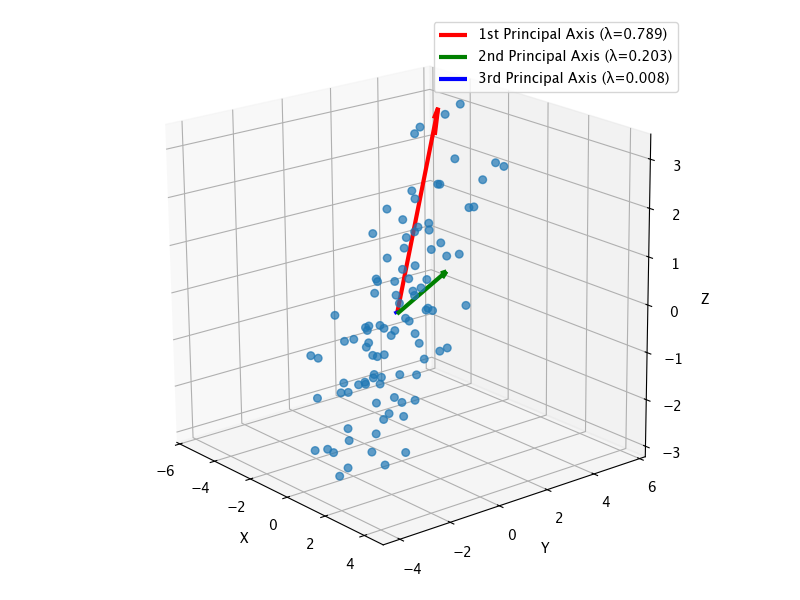
\includegraphics[scale=0.4]{img/pca_3d.png}
      \caption{We can see that the data approximately lies on a 2-dimensional subspace of $\mathbb{R}^3$.} 
    \end{figure}
  \end{example}

  \begin{example}[Eigenfaces]
    In 1991, Turk and Pentland presented an eigenface method of face recognition by taking the low-rank approximation of a dataset of face images \cite{1991turk}. 

    \begin{figure}[H]
      \centering 
      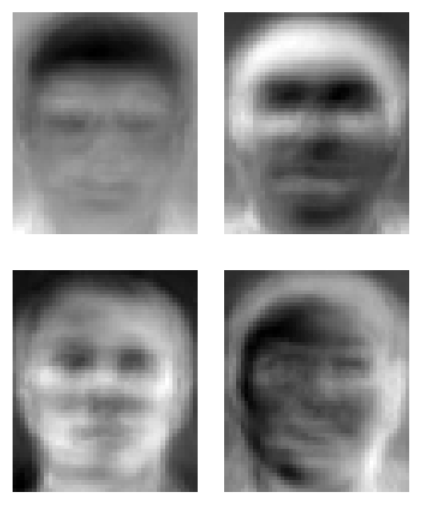
\includegraphics[scale=0.3]{img/eigenfaces.png}
      \caption{Some eigenfaces from AT\&T Labs. } 
      \label{fig:eigenfaces}
    \end{figure}
  \end{example}

  The first $k$ principal components provide not only the best rank $k$ approximation to $X$, but also the covariance matrix $\hat{\Sigma}$. 

  \begin{theorem}[PCA is an Unbiased Estimator of Sample Variance]
    The truncated covariance matrix $\Sigma^k = V_k S^2 V_k^T$ is an unbiased estimator of $X^T X$. 
  \end{theorem}
  \begin{proof}
    Indeed, $\hat{\Sigma} = X^T X = V S^2 V^T$, and the last equation is the SVD decomposition of $\hat{\Sigma}$. So again using Eckart-Young theorem, the best rank $k$ approximation to $\hat{\Sigma}$ is given by $\Sigma^k = V_k S^2 V_k^T$ (now truncated both in rows and columns). 
  \end{proof}

\subsection{Iterative Solvers} 

  A disadvantage of decomposition is that the time complexity of SVD on a $n \times m$ matrix is $O(nm \min\{n, m\})$. Therefore, we use iterative methods, which is really just applications of numerical linear algebra. 

\subsubsection{Power Method} 

  The simplest iterative eigenvalue solver was due to von Mises in 1929 \cite{1929vonmises}. Intuitively, given a diagonalizable matrix that we want to solve for, we can  ``normalize'' the spectrum by dividing all the eigenvectors by $\lambda_1$, the largest eigenvalue. Then by composing these linear maps, all the other eigenvectors should die out while keeping the largest eigenvector in place. 

  \begin{theorem}[Convergence of Power Iteration]
    Let $A \in \mathbb{R}^{n \times n}$ be a diagonalizable matrix and $x_0 \in \mathbb{R}^n$ any random vector. Given the two assumptions: 
    \begin{enumerate}
      \item $A$ has a unique greatest eigenvalue $\lambda_1$. 
      \item $x_0$ has a nonzero component in the direction of the eigenvalue $v_1$ associated with $\lambda_1$. 
    \end{enumerate}
    Then, the sequence $(x_t)$ by defined recursively as
    \begin{equation} 
      x_{t+1} = \frac{A x_t}{\|A x_t\|}
    \end{equation}
    converges to $v_1$. 
  \end{theorem}
  \begin{proof}
    We rewrite the recurrence relation as 
    \begin{equation}
    x_{t+1} = \frac{Ax_t}{\|Ax_t\|} = \frac{A^{t+1}x_0}{\|A^{t+1}x_0\|}
    \end{equation}

    Since $A$ is diagonalizable, we can write $A = VSV^{-1}$ where $V$ is the matrix of eigenvectors and $S$ is the diagonal matrix of eigenvalues. Thus:
    \begin{equation}
    x_t = \frac{A^t x_0}{\|A^t x_0\|} = \frac{(VSV^{-1})^t x_0}{\|(VSV^{-1})^t x_0\|} = \frac{VS^t V^{-1} x_0}{\|VS^t V^{-1} x_0\|}
    \end{equation}

    Since $x_0$ can be expressed as a linear combination of eigenvectors, we write $V^{-1}x_0 = c_1 e_1 + c_2 e_2 + \cdots + c_n e_n$ where $e_i$ are the standard basis vectors and $c_i$ are the coefficients. Therefore:
    \begin{align}
      x_t & = \frac{VS^t V^{-1}(c_1 v_1 + c_2 v_2 + \cdots + c_n v_n)}{\|VS^t V^{-1}(c_1 v_1 + c_2 v_2 + \cdots + c_n v_n)\|} \\ 
          & = \frac{VS^t(c_1 e_1 + c_2 e_2 + \cdots + c_n e_n)}{\|VS^t(c_1 e_1 + c_2 e_2 + \cdots + c_n e_n)\|}
    \end{align}

    Factoring out the dominant eigenvalue $\lambda_1$:
    \begin{equation}
      x_t = \left(\frac{\lambda_1}{|\lambda_1|}\right)^t \frac{c_1}{|c_1|} \frac{v_1 + \frac{1}{c_1}V\left(\frac{1}{\lambda_1}S\right)^t(c_2 e_2 + \cdots + c_n e_n)}{\left\|v_1 + \frac{1}{c_1}V\left(\frac{1}{\lambda_1}S\right)^t(c_2 e_2 + \cdots + c_n e_n)\right\|}
    \end{equation}

    Since $|\lambda_i/\lambda_1| < 1$ for $i > 1$, we have $\left(\frac{\lambda_i}{\lambda_1}\right)^t \to 0$ as $t \to \infty$. Therefore:
    \begin{equation}
    \frac{1}{c_1}V\left(\frac{1}{\lambda_1}S\right)^t(c_2 e_2 + \cdots + c_n e_n) \to 0 \text{ as } t \to \infty
    \end{equation}

    Thus, as $t \to \infty$:
    \begin{equation}
    x_t \to \left(\frac{\lambda_1}{|\lambda_1|}\right)^t \frac{c_1}{|c_1|} \frac{v_1}{\|v_1\|} = \pm v_1
    \end{equation}

    Since we assumed that $c_1 \neq 0$, the sequence $(x_t)$ converges to $\pm v_1$. 
  \end{proof}

  Therefore, a direct consequence of this theorem is. 

  \begin{algo}[Power Iteration to Solve Largest Eigenvector]
    Let $A \in \mathbb{R}^{n \times m}$. Then 
    \begin{algorithm}[H]
      \caption{Power Iteration Method}
      \label{alg:power_iteration}
      \begin{algorithmic}[1]
        \Procedure{PowerIteration}{$A$}
            
        \Require{$A \in \mathbb{R}^{n \times n}$ is a matrix, $max\_iter > 0$ is maximum iterations}
        
        \State $x \gets \text{ random vector of unit norm}$
        \State $\lambda \gets 0$
        
        \For{$t \gets 1$ to $max\_iter$}
          \State $y \gets Ax$
          \State $\lambda \gets x^T y$
          \State $x \gets \frac{y}{\|y\|}$
        \EndFor
        
        \State \Return $\lambda, x$
        \EndProcedure
      \end{algorithmic}
    \end{algorithm}
  \end{algo} 

  \begin{corollary}[Rate of Convergence of Power Iteration]
    The rate of convergence is 
    \begin{equation}
      \frac{\lambda_2}{\lambda_1}
    \end{equation}
  \end{corollary}

\subsubsection{Lanczos Algorithms} 

  The time complexity and the slow convergence of the power iteration led to faster algorithms, with one notable class being \textit{Lanczos algorithms}, first developed in 1950 \cite{1950lanczos}. 

  \begin{definition}[Krylov Subspace]
    Given linear map $A: V \to V$ and vector $v \in V$, the \textbf{$m$th Krylov subspace} is 
    \begin{equation}
      \mathcal{K}_m (A, v) = \mathrm{span} \{v, Av, A^2 v, \ldots, A^{m-1} v \}
    \end{equation}
  \end{definition}


  \begin{algo}[Lanczos Algorithm] 
    The basic idea is to construct an orthonormal basis for the Krylov subspace $\mathcal{K}_m (A, v)$ using a three term recurrence relation. This process transforms the original matrix $A$ into a tridiagonal matrix $T$ that can be used to compute the eigenvectors efficiently.  
    
    \begin{algorithm}[H]
      \caption{Lanczos Algorithm}
      \label{alg:lanczos}
      \begin{algorithmic}[1]
        \Procedure{Lanczos}{$A$, $m$}
            
        \Require{Hermitian matrix $A$ of size $n \times n$, number of iterations $m$ (default: $m = n$)}
        \Ensure{$n \times m$ matrix $V$ with orthonormal columns and tridiagonal real symmetric matrix $T = V^* A V$ of size $m \times m$}
        
        \State Let $v_1 \in \mathbb{C}^n$ be an arbitrary vector with Euclidean norm 1
        \State $w_1' \gets A v_1$
        \State $\alpha_1 \gets {w_1'}^* v_1$
        \State $w_1 \gets w_1' - \alpha_1 v_1$
        
        \For{$j \gets 2$ to $m$}
          \State $\beta_j \gets \|w_{j-1}\|$ (Euclidean norm)
          
          \If{$\beta_j \neq 0$}
            \State $v_j \gets w_{j-1} / \beta_j$
          \Else
            \State Pick $v_j$ as arbitrary vector with Euclidean norm 1 orthogonal to all of $v_1, \ldots, v_{j-1}$
          \EndIf
          
          \State $w_j' \gets A v_j - \beta_j v_{j-1}$
          \State $\alpha_j \gets {w_j'}^* v_j$
          \State $w_j \gets w_j' - \alpha_j v_j$
        \EndFor
        
        \State Let $V$ be the matrix with columns $v_1, \ldots, v_m$ and 
        \begin{equation}
          T = \begin{pmatrix}
            \alpha_1 & \beta_2 & & & \\
            \beta_2 & \alpha_2 & \beta_3 & & \\
            & \beta_3 & \alpha_3 & \ddots & \\
            & & \ddots & \ddots & \beta_{m-1} \\
            & & & \beta_{m-1} & \alpha_{m-1} & \beta_m \\
            & & & & \beta_m & \alpha_m
          \end{pmatrix}
        \end{equation}
        
        \State \Return $V, T$
        \EndProcedure
      \end{algorithmic}
    \end{algorithm} 

    For the runtime, 
    \begin{enumerate}
      \item Each iteration consists of an $O(nm)$ matrix multiplication with the rest of the operations $O(n)$. 
      \item If the matrix is sparse, then this is of order $O(nk)$, where $k$ is the average number of nonzero elements in each row. If $k$ is bounded, then we can compute each iteration in linear time $O(n)$. 
    \end{enumerate}
  \end{algo} 

  Now that we have $V, T$, what do we do? The following theorem tells us how to compute the original eigenvectors.  

  \begin{theorem}
    If $\lambda$ is an eigenvalue of $T$ and $x$ is its eigenvector (i.e., $Tx = \lambda x$), then $y = Vx$ is a corresponding eigenvector of $A$ with the same eigenvalue.
  \end{theorem}
  \begin{proof}
    Let $\lambda$ be an eigenvalue of $T$ with eigenvector $x$, so that $Tx = \lambda x$. We need to show that $y = Vx$ is an eigenvector of $A$ with eigenvalue $\lambda$.

    Since the Lanczos algorithm produces the relation $T = V^* A V$, we have $A = VTV^*$. Therefore:
    \begin{align}
      Ay &= AVx \\
         &= VTV^* Vx \\
         &= VTIx \\
         &= VTx \\
         &= V(\lambda x) \\
         &= \lambda Vx \\
         &= \lambda y
    \end{align}
  \end{proof}

  One note of warning. This algorithm tends to be numerically unstable and sometimes there is a loss of orthogonality among the Lanczos vectors due to finite precision arithmetic. We can however just reorthogonalize them in the end. 

\subsubsection{LOBPCG}

\subsubsection{NIPALS}

\subsubsection{Oja's Neuron}

  With neural networks on the rise, Oja developed a simple neuron function that can compute the greatest eigenvector \cite{1982oja}. Let's start with an extremely simple model of a neuron. 

  \begin{definition}[Neuron]
    Consider a linear model of a neuron that returns a sum of its inputs according to weighted presynaptic weights $y(x) = w^T x$. 
  \end{definition} 

  \begin{definition}[Hebb's Rule]
    In neuroscience, \textbf{Hebb's rule} (aka Hebbian learning) colloquially states that neurons are activated together have greater strengths, like how muscles grow when you work them more.\footnote{Neurons that fire together, wire together.}  
    \begin{equation}
      w_{t+1} - w_t = \eta y(x_t) x_t
    \end{equation}
  \end{definition}

  Since the weights are not constrained at all, we would find that the weights approach infinity if $\eta > 0$. Therefore, Oja resticted the weights so that the $p$-norm is $1$ , $0 \leq w_i \leq 1$, which models a form of competition for resources between the neurons \cite{1982oja}. Oja's mathematically formalized this rule in the following. 

  \begin{theorem}[Oja's Rule]
    Hebbian learning of a neuron can be modeled with
    \begin{equation}
      w_{t+1} - w_t = \eta y_t (x_t - y_t w_t)
    \end{equation}
    To parse this, let's focus on a component element $(x_t)_i$. If $x_t$ represents the neurons firing and $y_t w_t$ represents which neurons' wiring scaled by how much the overall neuron has fired, we want the $y_t w_t$ to move closer to $x_t$. Therefore, we update $w_t$ in the direction of this difference, and then scale it by $\eta y_t$. 
  \end{theorem}
  \begin{proof}
    Starting with Hebb's rule and applying normalization constraints, we have\footnote{Oja had $p = 2$ in his original paper, but in fact, any type of normalization, even linear, will give the same result without loss of generality.}
    \begin{equation}
      \mathbf{w}_{t+1} = \frac{\mathbf{w}_t + \eta y_t \mathbf{x}_t}{\left\|\mathbf{w}_t + \eta y_t \mathbf{x}_t\right\|_p}
    \end{equation}
    where $\|\mathbf{v}\|_p = \left(\sum_{j=1}^{m} |v_j|^p\right)^{1/p}$. For a small learning rate $|\eta| \ll 1$, we can expand this equation as a power series in $\eta$. Using the binomial approximation $(1 + \epsilon)^{-1/p} \approx 1 - \frac{\epsilon}{p}$ for small $\epsilon$, we get:
    \begin{equation}
      \mathbf{w}_{t+1} = \frac{\mathbf{w}_t}{\|\mathbf{w}_t\|_p} + \eta \left(\frac{y_t\mathbf{x}_t}{\|\mathbf{w}_t\|_p} - \frac{\mathbf{w}_t \mathbf{w}_t^T \mathbf{x}_t y_t}{\|\mathbf{w}_t\|_p^{p+1}} \|\mathbf{w}_t\|_p^{p-1}\right) + O(\eta^2)
    \end{equation}
   
    For small $\eta$, the higher-order terms $O(\eta^2)$ vanish. We specify a linear neuron where the output is:
    \begin{equation}
      y_t = \mathbf{x}_t^T \mathbf{w}_t^{(p-1)}
    \end{equation}
    where $\mathbf{w}_t^{(p-1)}$ denotes the component-wise power $[\mathbf{w}_t^{(p-1)}]_j = (w_t)_j^{p-1}$. We also specify that our weights are normalized: $\|\mathbf{w}_t\|_p = 1$. 
   
    For $p = 2$, this simplifies to $y_t = \mathbf{x}_t^T \mathbf{w}_t$ and $\|\mathbf{w}_t\|_2 = 1$. Substituting these conditions into our expansion gives:
    \begin{equation}
      \mathbf{w}_{t+1} = \mathbf{w}_t + \eta y_t(\mathbf{x}_t - y_t\mathbf{w}_t)
    \end{equation}
  \end{proof}

  Finally, we claim that $w_t$ asympototically converges to the first principal axes. 

  \begin{theorem}[Oja's Neuron Convergence to First Principal Component]
    Consider a single neuron trained by Oja's rule with weight vector $\mathbf{w}_t$ and input data $\{\mathbf{x}_t\}$ having correlation matrix $R = E[\mathbf{x}\mathbf{x}^T]$. Let $\mathbf{q}_1$ be the eigenvector corresponding to the largest eigenvalue $\lambda_1$ of $R$. Under the following conditions:
    \begin{enumerate}
      \item The learning rate $\eta(t)$ satisfies $\sum_{t=1}^{\infty} \eta(t) = \infty$ and $\sum_{t=1}^{\infty} \eta(t)^p < \infty$ for some $p > 1$
      \item The activation function $y(\mathbf{x}(t))$ is continuously differentiable in both $\mathbf{x}$ and $\mathbf{w}$ with bounded derivatives
      \item The correlation matrix $R$ has a unique largest eigenvalue $\lambda_1$
    \end{enumerate}
    Then the weight vector $\mathbf{w}_t$ converges to $\pm\mathbf{q}_1$ as $t \to \infty$, and the variance of the neuron's output converges to the principal eigenvalue:
    \begin{equation}
      \lim_{t \to \infty} \sigma^2(t) = \lim_{t \to \infty} \langle y^2(t) \rangle = \lambda_1
    \end{equation}
  \end{theorem}
  \begin{proof}
    TBD: Go over this. We analyze the convergence using Lyapunov function analysis. Consider the continuous-time version of Oja's rule:
    \begin{equation}
      \frac{d\mathbf{w}}{dt} = \eta(t) y(t) (\mathbf{x}(t) - y(t) \mathbf{w}(t))
    \end{equation}
    where $y(t) = \mathbf{w}(t)^T \mathbf{x}(t)$.
   
    Taking the expected value and assuming ergodicity of the input process:
    \begin{equation}
      \frac{d\mathbf{w}}{dt} = \eta(t) E[y(\mathbf{x} - y\mathbf{w})] = \eta(t) E[\mathbf{w}^T\mathbf{x}(\mathbf{x} - \mathbf{w}^T\mathbf{x}\mathbf{w})]
    \end{equation}
   
    This simplifies to:
    \begin{equation}
      \frac{d\mathbf{w}}{dt} = \eta(t) (R\mathbf{w} - \mathbf{w}^T R \mathbf{w} \mathbf{w})
    \end{equation}
   
    Since $\mathbf{w}$ is normalized ($\|\mathbf{w}\| = 1$), we have $\mathbf{w}^T R \mathbf{w} = \mathbf{w}^T R \mathbf{w}$. Let $\mathbf{w} = \sum_{i=1}^n c_i \mathbf{q}_i$ where $\{\mathbf{q}_i\}$ are the orthonormal eigenvectors of $R$ with eigenvalues $\{\lambda_i\}$ ordered as $\lambda_1 > \lambda_2 \geq \cdots \geq \lambda_n$.
   
    Substituting the eigendecomposition:
    \begin{equation}
      \frac{d\mathbf{w}}{dt} = \eta(t) \left(\sum_{i=1}^n c_i \lambda_i \mathbf{q}_i - \left(\sum_{i=1}^n c_i^2 \lambda_i\right) \sum_{j=1}^n c_j \mathbf{q}_j\right)
    \end{equation}
   
    For the coefficient $c_1$ corresponding to the first principal component:
    \begin{equation}
      \frac{dc_1}{dt} = \eta(t) c_1 \left(\lambda_1 - \sum_{i=1}^n c_i^2 \lambda_i\right)
    \end{equation}
   
    Since $\lambda_1$ is the largest eigenvalue and $\sum_{i=1}^n c_i^2 = 1$, we have $\lambda_1 - \sum_{i=1}^n c_i^2 \lambda_i > 0$ whenever $c_i \neq 0$ for $i > 1$.
   
    For $i > 1$:
    \begin{equation}
      \frac{dc_i}{dt} = \eta(t) c_i \left(\lambda_i - \sum_{j=1}^n c_j^2 \lambda_j\right)
    \end{equation}
   
    Since $\lambda_i < \lambda_1$, the term $(\lambda_i - \sum_{j=1}^n c_j^2 \lambda_j)$ becomes negative as $c_1$ grows, causing $c_i \to 0$ for $i > 1$.
   
    The conditions on $\eta(t)$ ensure convergence by the Robbins-Monro theorem: the divergent sum condition ensures the algorithm can reach any point in the space, while the convergent power sum condition ensures the noise diminishes sufficiently for convergence.
   
    As $t \to \infty$, we have $c_1 \to \pm 1$ and $c_i \to 0$ for $i > 1$, implying $\mathbf{w}_t \to \pm\mathbf{q}_1$.
   
    The variance of the output is:
    \begin{equation}
      \sigma^2(t) = E[y^2(t)] = E[(\mathbf{w}_t^T \mathbf{x}_t)^2] = \mathbf{w}_t^T R \mathbf{w}_t
    \end{equation}
   
    As $\mathbf{w}_t \to \pm\mathbf{q}_1$, we get:
    \begin{equation}
      \lim_{t \to \infty} \sigma^2(t) = \mathbf{q}_1^T R \mathbf{q}_1 = \lambda_1
    \end{equation}
  \end{proof}
 
  \begin{algo}[Oja's Rule]
    \begin{algorithm}[H]
      \caption{Oja's Neuron Algorithm}
      \label{alg:oja_neuron}
      \begin{algorithmic}[1]
        \Procedure{OjaNeuron}{$\mathbf{x}_1, \mathbf{x}_2, \ldots, \mathbf{x}_T$, $\eta$}
            
        \Require{Input data vectors $\mathbf{x}_t \in \mathbb{R}^n$ for $t = 1, 2, \ldots, T$, learning rate $\eta > 0$}
        \Ensure{Weight vector $\mathbf{w}$ that converges to the first principal component}
        
        \State Initialize $\mathbf{w}_0 \in \mathbb{R}^n$ randomly with small values
        
        \For{$t \gets 1$ to $T$}
          \State $y_t \gets \mathbf{w}_{t-1}^T \mathbf{x}_t$ \Comment{Neural output}
          \State $\mathbf{w}_t \gets \mathbf{w}_{t-1} + \eta y_t (\mathbf{x}_t - y_t \mathbf{w}_{t-1})$ \Comment{Oja's learning rule}
        \EndFor
        
        \State \Return $\mathbf{w}_T$
        \EndProcedure
      \end{algorithmic}
    \end{algorithm}
  \end{algo}

\subsection{The Importance of Standardizing} 

  Say that a covariate was a person's height in meters. If we had measured in centimeters, then the values would a hundred times higher. PCA does not account for this and so in most cases, you should standardize your data to have component-wise unit variance before. 

\subsection{Asymptotic Analysis}

  It turns out that the elements of $\hat{\Sigma}$ are close entry-wise to those of $\Sigma$. But if this is true, then does it mean that the eigenvalues of the sample covariance matrix are close to the true eigenvalues of the covariance matrix? It turns out that the answer is no, and we need a proper metric to satisfy this assumption. The metric, as we can guess from linear algebra, is the operator norm, and we will show some results from matrix perturbation theory. 

  \begin{lemma}[]
    It turns out that 
    \begin{equation}
      ||\hat{\Sigma} - \Sigma|| = O_p \bigg( \frac{1}{\sqrt{n}} \bigg)
    \end{equation}
    where $|| \cdot ||$ is the operator norm. 
  \end{lemma}

  \begin{theorem}[Weyl's Theorem]
    If $\hat{\Sigma}$ and $\Sigma$ are close in the operator norm, then their eigenvalues are close. 
    \begin{equation}
      ||\hat{\Sigma} - \Sigma|| = O_p \bigg( \frac{1}{\sqrt{n}} \bigg) \implies |\hat{\lambda}_j - \lambda_j| = O_p \bigg( \frac{1}{\sqrt{n}} \bigg) 
    \end{equation}
  \end{theorem}

  This only talks about their eigenvalues, but this does not necessarily imply that the eigenvalues are close. We need an extra condition. 

  \begin{theorem}[David-Kahan Theorem]
    If $\hat{\Sigma}$ and $\Sigma$ are close in the operator norm, and if the eigenvectors of $\Sigma$ are well-conditioned, then the eigenvectors of $\hat{\Sigma}$ are close to the eigenvectors of $\Sigma$. More specifically, 
    \begin{equation}
      ||\hat{v}_j - v_j|| \leq \frac{2^{3/2} ||\hat{\Sigma} - \Sigma||}{\lambda_j - \lambda_{j+1}}
    \end{equation}
  \end{theorem}



